\documentclass[12pt, a4paper]{memoir}

% Essential packages
\usepackage[T1]{fontenc}
%%\usepackage[latin1]{inputenc}
\usepackage[french,english]{babel}

% personal packages
\usepackage [includehead, margin=1.5cm]{geometry}                % See geometry.pdf to learn the layout options. There are lots.
\usepackage{graphicx} % include images
\usepackage{hyperref} % urls, hyperlinks, etc
% \usepackage{pdfpages} % include pdf pages
\usepackage{enumitem} % customize itemize
\usepackage[backend=bibtex]{biblatex} % bibliography
\usepackage{csquotes} % Quote bibliography and add hyperlinks
% \usepackage{titlesec} % Modify chapter headings
% \usepackage{wrapfig} % wrap text around figures
% \usepackage{float} % force figure positions at the end of the file
\usepackage[linesnumbered,ruled,vlined]{algorithm2e}

% Packages from uga template
%\usepackage{fullpage}
\usepackage{mathptmx} % font = times
\usepackage{helvet} % font sf = helvetica
% \usepackage{amsmath}
% \usepackage{relsize}
% \usepackage{tikz}
% \usepackage{booktabs}
% \usepackage{textcomp}%textquotesingle
% \usepackage{multirow}
%
\usepackage{minted}

% \usetikzlibrary{arrows,shapes,positioning,shadows,trees}
% \makesavenoteenv{tabular}
% \makesavenoteenv{table}

\def\checkmark{\tikz\fill[scale=0.4](0,.35) -- (.25,0) -- (1,.7) -- (.25,.15) -- cycle;}

%Style des têtes de section, headings, chapitre
\headstyles{komalike}
\nouppercaseheads
\chapterstyle{dash}
\makeevenhead{headings}{\sffamily\thepage}{}{\sffamily\leftmark} 
\makeoddhead{headings}{\sffamily\rightmark}{}{\sffamily\thepage}
\makeoddfoot{plain}{}{}{} % Pages chapitre. 
\makeheadrule{headings}{\textwidth}{\normalrulethickness}
%\renewcommand{\leftmark}{\thechapter ---}
\renewcommand{\chaptername}{\relax}
\renewcommand{\chaptitlefont}{ \sffamily\bfseries \LARGE}
\renewcommand{\chapnumfont}{ \sffamily\bfseries \LARGE}
\setsecnumdepth{subsection}
\addbibresource{biblio.bib}

% Customize itemize item markers
\renewcommand\labelitemi{-}

% Add source to figures caption
\newcommand*{\captionsource}[2]{%
    \caption[{#1}]{%
        #1%
        \\\hspace{\linewidth}%
	\textbf{Source:} \textit{#2}%
    }%
}

% Some settings for the title page
%\titleformat{\chapter}[display]{\normalfont\huge\bfseries}{}{0pt}{\Huge}
%\titlespacing*{\chapter} {0pt}{20pt}{40pt}

% Force footnotes to stay on one page
\interfootnotelinepenalty=10000

% Title page formatting -- do not change!
\newcommand{\HRule}{\rule{\linewidth}{0.5mm}}
\pretitle{\HUGE\sffamily \bfseries\begin{center}\HRule \\[0.2cm]} 
	\posttitle{\end{center}\HRule}
\preauthor{\LARGE  \sffamily \bfseries\begin{center}}
\postauthor{\par\end{center}}
\newcommand{\jury}[1]{% 
\gdef\juryB{#1}} 
\newcommand{\juryB}{} 
\newcommand{\session}[1]{% 
\gdef\sessionB{#1}} 
\newcommand{\sessionB}{} 
\newcommand{\option}[1]{% 
\gdef\optionB{#1}} 
\newcommand{\optionB} {}

\renewcommand{\maketitlehookd}{% 
\vfill{}  \large\par\noindent  
\begin{center}\juryB \bigskip\sessionB\end{center}
\vspace{-1.5cm}}
\renewcommand{\maketitlehooka}{% 
	\vspace{-1.5cm}\noindent
\includegraphics[height=10ex]{./imgs/uga-logo.png}\hfill
\includegraphics[height=10ex]{./imgs/ryax-logo.png}\hfill
\includegraphics[height=10ex]{./imgs/Logo-LIG.jpg}\hfill
\includegraphics[height=12ex]{./imgs/ENSIMAG.png}
\bigskip
\begin{center} \large
Master of Science in Informatics at Grenoble \\
Master Informatique \\ 
Specialization \optionB  \end{center}\vfill}
% =======================End of title page formatting

\option{MoSIG} 
\title{Simulation of a Kubernetes Cluster with Validation in Real Conditions} %\\\vspace{-1ex}\rule{10ex}{0.5pt} \\sub-title} 
\author{LARUE Théo}
\date{Defense Date, 2020} % Delete this line to display the current date
\jury{
	Research project performed at Laboratoire d'Informatique de Grenoble \\\medskip
Under the supervision of:\\
Michael Mercier\\\medskip
Defended before a jury composed of:\\
Head of the jury\\
Jury member 1\\
Jury member 2\\
}
\session{September \hfill 2020}
\setcounter{tocdepth}{4}
\setcounter{secnumdepth}{4}

\begin{document}
\selectlanguage{english} % french si rapport en français
\frontmatter
\begin{titlingpage}
\maketitle
\end{titlingpage}

%\small
\setlength{\parskip}{-1pt plus 1pt}

\renewcommand{\abstracttextfont}{\normalfont}
\abstractintoc
\begin{abstract} 
	TODO : rework this with the new intro


	The rise of containerized applications has provided web platforms with
	much more control over their resources than they had before with their
	physical servers. Soon enough, developers realized they could go even
	further by automating container management operations to allow for even
	more scalability. The Cloud Native Computing Foundation was founded in
	this context, and developed Kubernetes which is a piece of software
	capable of container orchestration, or in other words, container
	management. Now, as we observe a convergence between HPC (High
	Performance Computing) and the Big Data field where Kubernetes is
	already the standard for some applications such as Machine Learning,
	discussions about leveraging containers for HPC applications rose and
	interest in Kubernetes has grown in the HPC community. One of the many
	challenges the HPC world has to face is scheduling, which is the act of
	allocating tasks submitted by users on available resources. In order to
	properly evaluate and develop schedulers researchers have used
	simulators for decades to avoid running experiments in real conditions,
	which is costly both in time and resources. However, such simulators do
	not exist for Kubernetes or are not open to the public. While the
	default scheduler works great for most of the Cloud Native
	infrastructures Kubernetes was designed for, some teams of researchers
	would rather be able to experiment with different batch processing
	policies on Kubernetes as they do with traditional HPC. Our goal in
	this master thesis is to describe how we developed Batkube, which it is
	an interface between Kubernetes schedulers and Batsim, a general
	purpose infrastructure simulator based on the Simgrid framework and
	developed at the LIG.

\end{abstract}
\abstractintoc

\renewcommand\abstractname{Acknowledgement}
\begin{abstract}
I would like to express my sincere gratitude to .. for his invaluable assistance and comments in reviewing this report... 
Good luck :) 
\end{abstract}

\renewcommand\abstractname{R\'esum\'e}
\begin{abstract} \selectlanguage{french}
	Abstract mais en franchais
\end{abstract}
\selectlanguage{english}

\tableofcontents* % the asterisk means that the table of contents itself isn't put into the ToC
\normalsize

\mainmatter
\SingleSpace

\chapter{Introduction}

TODO: Make another pass on that section after everything else is redacted (or
at least the soa)\\

The need for scalable computing infrastructure has increased tremendously in
the last decades. Nearly every field of computer science, from research to the
service industry, now needs a proper infrastructure and by 2025, computation
technology could reach a fourth of the global electricity
spending\cite{andrae2017total}.  Even the public sector is now in need for
efficient distributed infrastructure as the concept of smart cities is
developing.

Organizations generally know what type of infrastructure will meet their needs.
It can take the form of Big Data centers to store and analyze data,
High-Performance Computers for computing intensive tasks or GPU banks for
machine learning or crypto-currency mining.  However, studying those
infrastructures extensively is much more challenging.  As these computers reach
scales in the order of warehouses\cite{barroso2018datacenter}, quantifying a
system's performance under varying loads, applications, scheduling policies and
system size quickly becomes undoable without expensive real world experiments.
In fact, the nature of scheduling problems\cite{scheduler-complexity} alone
make theoretical studies hard.  This is an issue for organizations as they rely
on thoses studies to determine the size of the required system or choose
optimal scheduling
policies.\\

Simulation allows to tackle these issues by enabling users to draw conclusions
empirically without the need to fire up real workloads. Indeed, running an
entire experimental campaign on a real system represents consequencial costs
both in time and money. With simulation, The gain in both time and spent energy
can be extreme : a HPC job spanning months on a real system can be resolved in
a matter of minutes on any domestic computer.  Another major point is that it
also brings reproducibility to these experiments, that otherwise would have to
be run on the exact same systems as their first iteration. With simulation, one
can recreate the same conditions for any experiment anywhere they want, and
expect the same results.\\

However, simulations need to be run with sound models for the results to be
exploitable and in that regard, simulators usually fall under several
pitfalls\cite{poquet:tel-01757245}. Very often simulators are implemented at
the same time as new schedulers or Resource and Jobs Management
Systems\footnote{The RJMS is the software at the core of the cluster. It is a
synonym for a scheduler and manages resources, energy consumption, users' jobs
life-cycle and implements scheduling policies.} in order to validate their
algorithms. Thus, they are strongly coupled together and are not usable with
any other software. They are either shipped with the software itself or worst,
they are never released and discarded at the end of the development process.
Moreover, still according to \cite{poquet:tel-01757245}, strong coupling may
lead to unrealistic models. In that case cluster resources can be accessed with
ease by the scheduler, resulting in it having very precise information about the
system state to take its decisions.  This conflicts with the real world as a
scheduler may not have access to all the information it wants, or may suffer
from latency when getting it from the system.\\

To try and assess these issues a team of researchers at the LIG developed
Batsim\cite{dutot:hal-01333471} which is a general purpose infrastructure
simulator with modularity and separation of concerns in mind. Batsim is based
on SimGrid\cite{casanova:hal-01017319} which is a framework for developing
simulators for distributed computer systems. Simgrid is now a 20 years old
framework that has been used in many
projects\footnote{https://simgrid.org/usages.html}, making it a sound choice to
run scalable and accurate models of the reality.

Batsim was designed to support algorithms written in any languages, as long as
they support its communication protocol. It means that, while any scheduler
found in the wild can potentially be run on a Batsim simulation, they still
have to be adapted to make them compatible. This master's project is dedicated
on developing an interface between Batsim and
Kubernetes\footnote{https://github.com/kubernetes/kubernetes/} schedulers in
order to run Kubernetes clusters simulations. Kube\footnote{Another term to
designate Kubernetes. It is also sometimes called k8s.} is an open source
container management software widely exploited in the industry for its ease of
use and wide range of capabilities. It has freed developers from the cumbersome
task of setting up low level software infrastructure on their servers and
automates maintenance, scaling and administration of their applications. For
all these reasons it has become a de-facto solution for any organization that
wishes to build new internet platforms from the ground up.\\

TODO : what we where able to do (summary of the simulator capabilities,
experimentations, results)

\chapter{State of the art}

This section is organized as follow. First we put Kubernetes in context, in
light of the advances made in web application development. As we will see,
despite these adavances in the automation of resource management many
fundamental questions remain that can only be anwsered by extensive studies on
computer systems. One such question is the problem of scheduling tasks on
compute resources, which we briefly present. We end this section by presenting
the concepts of Batsim which is a distributed system simulator especially well
suited for studies on scheduling alrogithms.

\section{Cloud Computing}

In the early stages of application development, organizations used to run their
services on physical servers. With this direct approach came many challenges
that needed to be coped with manually like resources allocation,
maintainability or scalability. In an attempt to automate this process
developers started using virtual machines which enabled them to run their
services regardless of physical infrastructure while having a better control
over resource allocation.  This led to the concept of containers which takes
the idea of encapsulated applications further than plain virtual machines.

\begin{figure}[h]
	\centering
	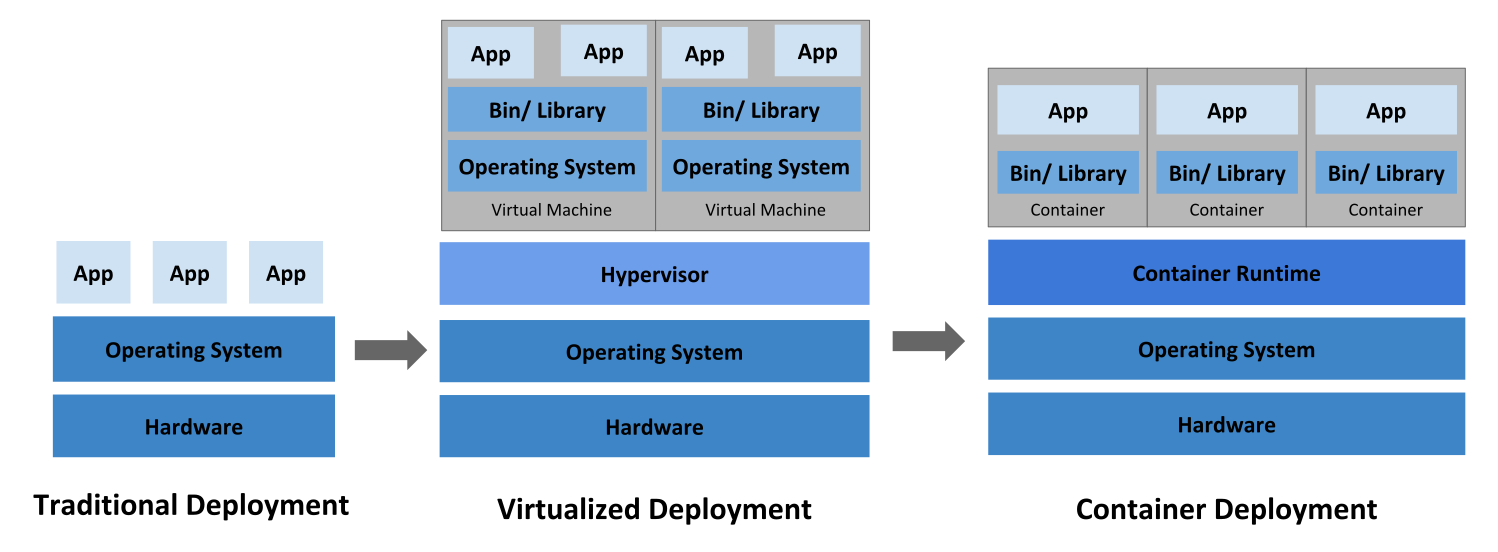
\includegraphics[width=\textwidth]{./imgs/container_evolution.png}
	\captionsource{Evolution of application deployment.}{https://kubernetes.io/docs/concepts/overview/what-is-kubernetes/}
	\label{fig:container-evolution}
\end{figure}

Containers can be thought of as lightweight virtual machines. Unlike the
latter, containers share the same kernel with the host machine but still allow
for a very controlled environment to run applications. There are many
benefits to this : separating the development from deployment, portability,
easy resource allocation, breaking large services into smaller micro-services
or support of continuous integration tools (containers greatly facilitate
integration tests).\\

The CNCF\footnote{\url{https://www.cncf.io/}} (Cloud Native Computing
Foundation) was founded in the intent of leveraging the container technology
for an overall better web. In a general way, we now speak of these
containerized and modular applications as cloud native computing :

\textit{``Cloud native technologies empower organizations to build and run
	scalable applications in modern, dynamic environments such as public,
	private, and hybrid clouds. Containers, service meshes, microservices,
	immutable infrastructure, and declarative APIs exemplify this
	approach.}

\textit{These techniques enable loosely coupled systems that
	are resilient, manageable, and observable.  Combined with robust
	automation, they allow engineers to make high-impact changes frequently
	and predictably with minimal toil.``}\footnote{\url{https://github.com/cncf/toc/blob/master/DEFINITION.md}}

Kubernetes\footnote{\url{https://kubernetes.io/}} is the implementation of this
general idea and was anounced at the same time as the CNCF. It aims at
automating of the process of deploying, maintaining and scaling containerized
applications. It is industry grade and is now the de-facto solution for
container orchestration.



\section{Studying computer infrastructures} \label{study-computing-infra}

Eventhough this paradigm enabled developing new applications with ease, many
questions remain: what type of infrastructure would be best suited for my
application? Would my application benefit from more cpu cores? How would
different scheduling policies affect my application? Would my batch jobs
compute faster with a different topology? To answer these interrogations one
must conduct studies to experiment with different configurations.\\

Studying an entire computing infrastructure is not an easy feat, first because
every infrastructure is unique. There are as many types of infrastructure as
there are use cases, each having a different vision on efficiency and what
metrics are critical to the system: latency, bandwith, resource availability,
computational power or cost effectiveness (the latter boils down to energy
efficiency). This variety of purposes translates to the type of hardware used
and the topology of the infrastructure. Some systems are centralized like HPC
and Data Centers, others are meant to be used from a distance like Cloud
Computing infrastructures and others are decentralized like Grid Computing,
Volunteer Computing and Peer to Peer computing. There are as many systems as
there are objectives to be achieved.

As a consequence, there are no general tools to study those systems.
Furthermore, as the biggest supercomputers are approaching the exascale
barrier\footnote{https://www.top500.org/news/japan-captures-top500-crown-arm-powered-supercomputer/}
and consist of thousands of nodes with millions of cpu cores (more than 7M for
the new ``Fugaku'' Japanese supercomputer), no human would be capable of
building a general mathematical model that would be accurate enough to predict
the behavior of those systems under varying conditions. Also, interactions
between the various components of those systems may lead to unexpected
behavior\cite{10.1007/978-3-319-09873-9_12} that can hardly be predicted.

In order to extensively experiment on a given system, there are 3 options left
as described in\cite{legrand2015scheduling}: \textit{in vivo}, \textit{in
vitro} and \textit{in silico} studies, which correspond respectively to
experiments on real testbeds, emulation and simulation.  

The next parts are mostly built upon \cite{legrand2015scheduling} and
\cite{casanova:hal-01017319} and are aimed at depicting the current landscape
of experimentation on distributed systems.

\subsubsection{\textit{in vivo} and \textit{in vitro} studies}

The most direct approach to study an infrastructure is running \textit{in vivo}
experiments, that is to say running experiments on a real testbed. This will
produce the most accurate results, however it poses major scalability and
reproducibility issues.

Experiments conducted on real systems may prove difficult to reproduce, as one
must have access to the same system to reiterate it. Even then, changes to the
infrastructure hardware and software environment diminish the chances of
getting the same conditions. One solution to this problem is running \textit{in
vitro} studies, that is to say run an emulation of the system (virtual machines
or a network emulation for example). This resolves the issue of
reproducibility, however the matter of the cost in energy and time remains (if
anything, emulation aggravates these costs).

This cost is exacerbated by the many iterations of a same experiment one must
conduct in order to get statistically significant results. Workloads submitted
by real users can last from hours to months and have substantial costs in
energy: the means required to run them are too great and research to optimize
or simply study these systems can not justify this waste of resources. For all
these reasons scientists resort to simulation to study these computing
infrastructures.

\subsubsection{\textit{in silico} studies, or simulation}

When running simulations two primary concerns are accuracy and scalability.
Accuracy is the measure of the bias between the simulated trace of an execution
of an application and its trace as if it were executed on a real system (the
lower it is, the higher the accuracy). Scalability is the ability of the
simulator to compute simulations quickly, or run large scale experiments.\\

Problems with simulation: often unrealeased simulators, or designed for a
specific project, or short lived (OptorSim) -> This is why Batsim was created.

Simulators specific to platforms: YARNSim, SLURM simulator\footnote{https://github.com/ubccr-slurm-simulator/slurm\_simulator} 
Exemples of papers with custom unreleased simulators: \cite{yabuuchi2019lowlatency} by the same guys who made kubernetes-simulator.\\

list of simulators
\begin{itemize}
	\item SimGrid, GridSim, CloudSim, GroudSim (to cite the most important).
	\item Other simulators in unrelated domains: SimBA (volunteer computing), PeerSim, OverSim (peer to peer), WRENCH (workflows).
	\item HPC simulation: off-line vs on-line
	\item Interconnected networks Simulation: INSEE (environment for interconnected networks), SICOSYS. Aimed to be used with other tools like SIMICS to extend th ecapabilities.
	\item Low level simulation: SIMICS, RSIM and SimOS (multiprocessor systems).
	\item discontinued/old projects: GSSIM, Simbatch
\end{itemize}

\subsubsection{Kubernetes simulation}

Kubernetes simulation: k8-cluster-simulator, joySim.


\section{The scheduling problem}

In particular, this work is targeted at experimenting with scheduling in a
distributed system driven by Kubernetes. Here we present a general definition
of scheduling, and the challenges it tackles.

\begin{displayquote}[][]
	\textbf{schedule} \textit{n.} : A plan for
	performing work or achieving an objective, specifying the order and
	allotted time for each part.
\end{displayquote}

In a general way, scheduling is the concept of allocating available resources
to a set of tasks, organizing them in time and space (the resource space). The
resources can be of any nature, and the tasks independent from each others or
linked together.

In computing the definition remains the same, but with automation in mind.
Schedulers are algorithms that take as an input either a pre-defined workload,
which is a set of jobs  to be executed, or single jobs submitted over time by
users in an unpredictable manner (as it is most often the case with HPC for
example). In the latter case, the jobs are added to a queue managed by the
scheduler. Scheduling is also called batch scheduling or batch processing, as
schedulers allocate batches of jobs at a time. Jobs are allocated on machines,
virtual or physical, with the intent of minimizing the total execution time,
equally distributing resources, minimizing wait time for the user or reducing
energy costs. As these objectives often contradict themselves so schedulers have
to implement compromises or focus on what the user requires from the system.

The scheduler has many factors to keep in mind while trying to be as efficient
as possible, such as:

\begin{itemize}
	\item Resource availability and jobs resource requirements
	\item Link between jobs (some are executed in parallel and need synchronization, some are independent)
	\item Latency between compute resources
	\item Compute resources failures
	\item User defined jobs priority
	\item Machine shutdowns and restarts
	\item Data locality
\end{itemize}

All these elements make scheduling a very intricate problem that is at best
polynomial in complexity, and often NP-hard (\cite{10.1016/S0022-0000(75)80008-0}, \cite{scheduler-complexity}).

\subsection{How to study this problem in particular}
Some simulators are especially well suited for this.
Aléa and Accasim, and Batsim, which is what we build upon.

\section{Batsim concepts}

Batsim\cite{dutot:hal-01333471} is a distributed system simulator built upon
the SimGrid framework. Its main objective is to enable the study of RJMS
without the need to implement a custom simulator, by providing a universal text
based interface. In this section we first present the SimGrid framework and then we present some of the core concepts and objectives of Batsim.

\subsubsection{SimGrid}

To understand Batsim's paradigms and view on simulation, we first need to
present Simgrid's paradigms. As the latter is the framework that Batsim builds
upon, Batsim and Simgrid views on simulation cannot be distinguished.

TODO

\subsubsection{Batsim}

Batsim is entirely deterministic so at to make the studies easily reproducible.
Its event-based models will provide the same results given the same inputs and
decision process. One other way Batsim facilitates reproducibility is through
its user-defined inputs. Unlike other HPC or grid computing simulations that
run on existing application traces, Batsim takes a user defined workload as an
input. As a consequence, the user has no concerns such as intellectual property
on application traces and may provide all his experiments materials and
environment.  Another advantage of this system is that the user can adapt the
workload depending on its needs, to achieve different levels of realism.

Batsim, just like SimGrid, aims at being versatile. The common belief is that
specialization is the key to achieving realistic results, however according to
SimGrid this versatility is all but an obstacle to
accuracy\cite{casanova:hal-01017319}: it is on the contrary the key to their
results which are both scalable and accurate. Batsim computation platforms are
SimGrid platforms meaning that theoretically, they may be as broad as SimGrid
allows it. In reality any SimGrid platform is not a correct Batsim platform.
Because Batsim aims at studying RJMS software, it requires a \textbf{master}
node that will host the decision process. The other hosts (or computational
resources) will have either the roles of \textbf{compute\_node} or
\textbf{storage}. Still, the user may study any topology he wishes using
SimGrid models.

Thanks to its own message interface based on Unix sockets, Batsim is language
agnostic which means that any RJMS can be plugged into it as long as it
implements the interface.

TODO: why batsim?

Because it was developed at the lig and they want to expand its capabilities.
It is language agnostic to very convenient to work with.

\chapter{Integrating the simulator into Kubernetes ecosystem}

\section{Problematic}

Batsim is able to run simulations of any distributed system, to study any
event-based scheduler that would implement its message protocol. Kubernetes is
a piece of software where all its component, including the scheduler, revolve
around a central API. Everything is then asynchronous as the API can be
accessed anytime by any component.

The question that arises is, can we adapt Batsim to make it support Kubernetes
schedulers? In other words, is it possible to implement an adaptive layer
between a synchronous event based simulator like Batsim and a scheduler
implemented following the asynchronous paradigms of APIs?

It will follow that in order to do so, we re-implemented an API following
Kubernetes API specifications and intercepted the scheduler's time to
synchronize it with the simulation time. This allows us to run lengthy
workloads in seconds using a scheduler otherwise supposed to rely on ``real''
machine time. We first describe some technical concepts about Kubernetes and
Batsim, and then describe how we re-implemented the API, intercepted the time,
and handled the synchronization of the different times between Batsim and the
scheduler.

\section{Batsim concepts}

\section{Kubernetes concepts}

The basic processing unit of Kubernetes is called a \textbf{pod} which is
composed of one or several containers and volumes\footnote{A volume is some
	storage space on the host machine that can be linked to containers, so
	they can read persistent information or store data in the long term}.
In the cloud native context a pod most often hosts a service or micro-service.

\begin{figure}[h]
	\centering
	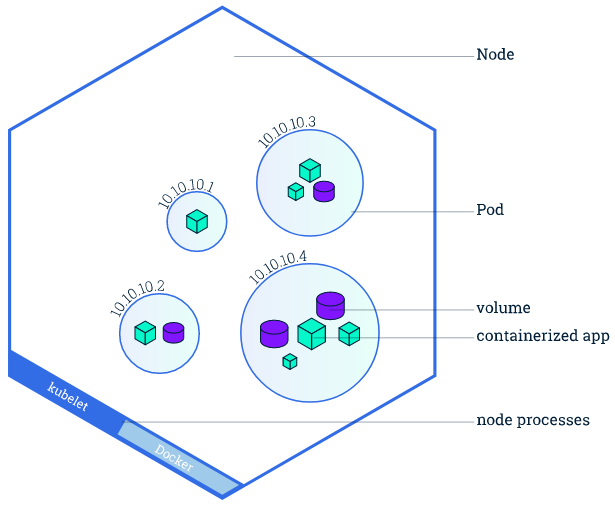
\includegraphics[scale=0.5]{./imgs/node-overview.png}
	\captionsource{Node overview}{https://kubernetes.io/docs/tutorials/kubernetes-basics/explore/explore-intro/}
	\label{fig:node-overview}
\end{figure}

Pods are bundled together in \textbf{nodes} (figure \ref{fig:node-overview})
which are either physical or virtual machines. They represent another barrier
to pass through to access the outside world which can be useful to add layers
of security or facilitate communication between pods. Nodes take the idea of
containerisation further by encapsulating the already encapsulated services.
Each node runs at least one pod and also one \textbf{kubelet} which is a
process responsible for communicating with the rest of Kubernetes (or more
precisely, with the master node which in turns communicates with the api
server). A set of nodes is called a \textbf{cluster}. Each Kubernetes instance
is responsible for running a cluster.

Kubernetes revolves its API server which is its central component (figure
\ref{fig:kube-components}). The majority of operations between components go
through this REST API like user interactions through kubectl or scheduling
operations.

\begin{figure}[h]
	\centering
	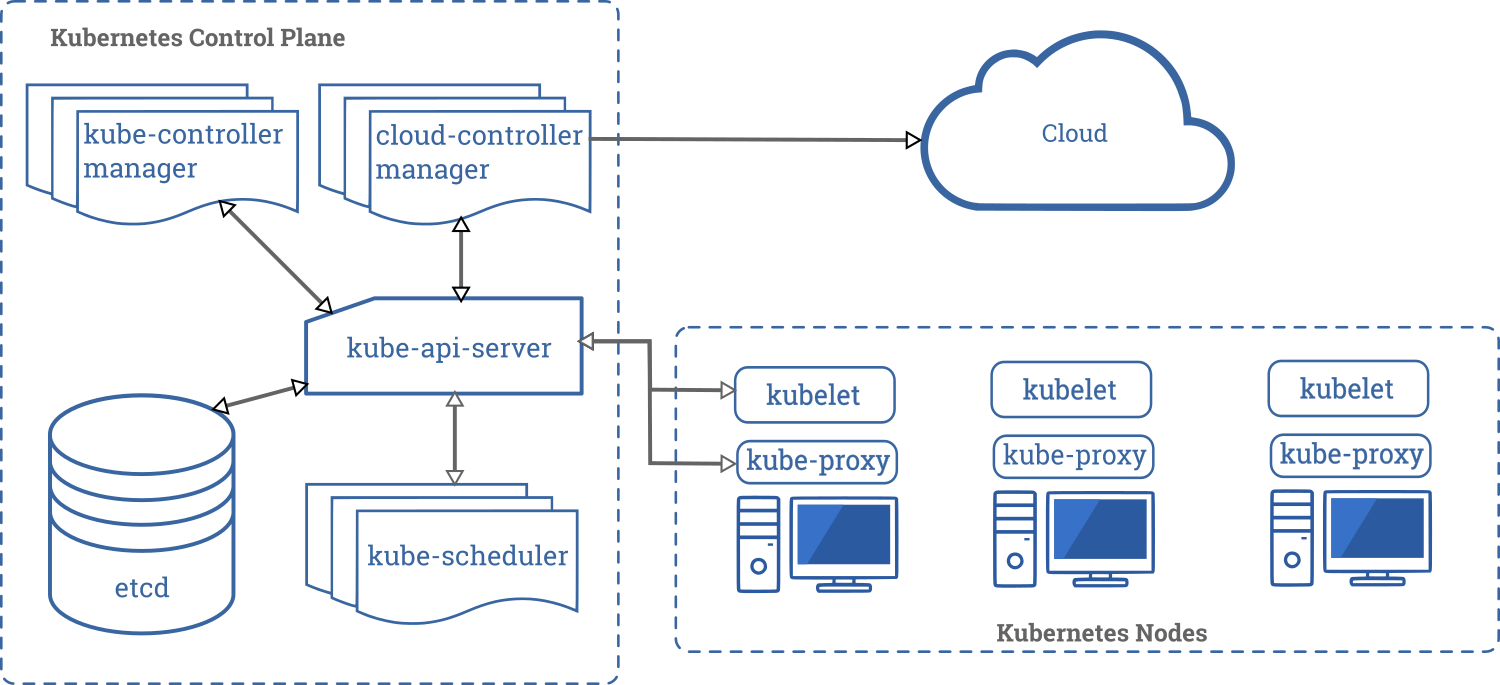
\includegraphics[width=\textwidth]{./imgs/components-of-kubernetes.png}
	\captionsource{Components of Kubernetes}{https://kubernetes.io/docs/concepts/overview/components/}
	\label{fig:kube-components}
\end{figure}

%\subsection{HPC and Kubernetes}
%The difference between HPC and Cloud Native computing lies in the workloads
%they are intended to tackle.  Kubernetes was designed for Cloud Native
%applications. Services or micro services are run in containers and are expected
%to be available at all times : they are replicated as many times as the user
%desires and restarted whenever a failure occurs. High availability is at the
%core of Kubernetes container management.  On the other hand, depending on
%scheduling policies, HPC is focused on user wait time, maximizing resource
%usage, optimizing energy costs... For instance, in case of failure, it is
%sometimes not sufficient to restart the single job that failed : the entire
%submission must be re-run if it is part of several jobs computed in parallel.
%
%Kubernetes is now the standard for AI and Machine Learning as shown by the many
%efforts at making this coupling an efficient
%environment\cite{lee2017design}\cite{233001}\cite{10.1145/3154842.3154845},
%which brought an increasing interest for container driven HPC aswell and
%Kubernetes for HPC in particular. Batch schedulers such as
%kube-batch\footnote{\url{https://github.com/kubernetes-sigs/kube-batch}} have
%been implemented for kube, and numerous HPC applications like
%slurm\footnote{\url{https://slurm.schedmd.com/containers.html}} now support containers as well.
%
%Indeed, containers have many advantages that HPC users can benefit from. Here
%are some notable ones:
%\begin{itemize}
%	\item First off, research has shown that Kuberenetes offer similar
%		performance to more standard bare metal HPC\cite{8950981}.
%	\item Users will get the same environment everywhere making up for a
%		uniform and standardized workplace.
%	\item Portability : users could seamlessly hop from one infrastructure
%		to another based on their needs and criteria like price,
%		performance, and capabilities rather than compatibility.
%	\item Encapsulation : HPC applications often rely on complex
%		dependencies that can be easily concealed into containers.
%\end{itemize}
%\begin{figure}[h]
%	\centering
%	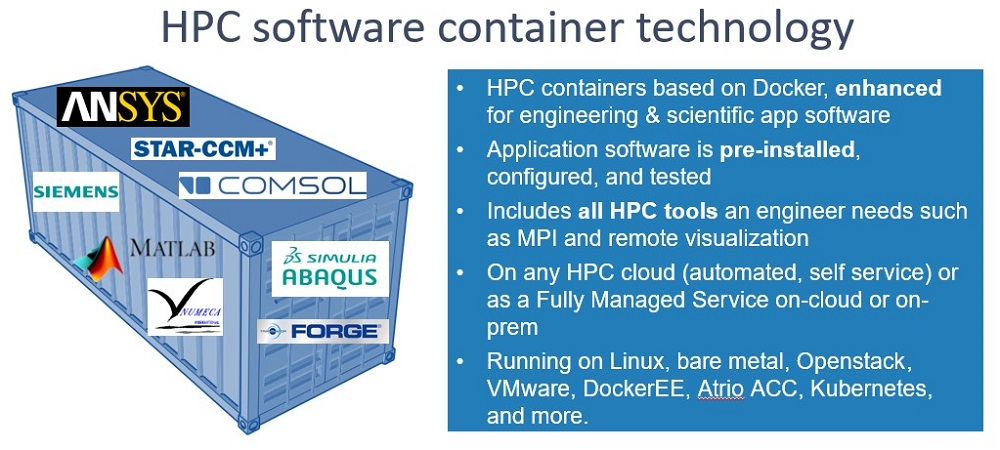
\includegraphics[scale=0.5]{./imgs/hpc-container.jpg}
%	\captionsource{The container technology for HPC}{https://www.hpcwire.com/2019/09/19/kubernetes-containers-and-hpc/}
%	\label{fig:hpc-container}
%\end{figure}
%
%Despite all those advantages, Kubernetes is not ready yet to be used in proper
%HPC environment because it lacks vital components like a proper batch job
%queuing system, and support for MPI applications. It cannot yet compete against
%the very well established HPC ecosystem, but that time may come soon as
%containers are becoming more and more integrated in modern infrastructures.



\section{Technical challenges}
\subsection{Translation}
\subsection{Time interception}
TODO

%\SetKwInput{KwInput}{Input}
%\SetKwInput{KwOutput}{Output}
%
%
%\begin{algorithm}[H]
%\DontPrintSemicolon
%\KwInput{req: request channel, res: result channel map}
%\While{Batkube is not ready} {
%	wait\;
%}
%requests = []request\;
%\While{req is not empty} {
%	m = $<$- req \tcc{Non blocking receive}
%	requests = append(requests, m)\;
%}
%sendToBatkube(requests) \tcc{Only requests with duration > 0 are actually sent. Batkube will always anwser.}
%now = responseFromBatkube()\;
%\For{m in range requests} {
%	res[m.id] $<$-now \tcc{The caller continues execution upon reception}
%}
%
%	
%\caption{Requester loop}
%\label{alg:reqLoop}
%\end{algorithm}
%
%
%\begin{algorithm}[H]
%\DontPrintSemicolon
%\KwResult{Current simulation time}
%\KwInput{d: timer duration, req: request channel, res: response channel map}
%\KwOutput{now : simulation time}
%
%\If{requester loop is not running}{
%	go runRequesterLoop() \tcc{There can on ly be one loop runing at a time}
%}
%id = newUUID()\;
%m = newRequestMessage(d, id) \tcc{Requests are identified using uuids}
%resChannel = newChannel()\;
%res[id] = resChannel \tcc{A channel is associated with each request}
%req $<$- m \tcc{The code blocks here until request is handled}
%now = $<$-resChannel \tcc{The code blocks here until response is sent by the requester loop}
%return now\;
%\caption{Time request (time.now())}
%\label{alg:now}
%\end{algorithm}


\subsection{Time synchronisation}

%\begin{algorithm}[H]
%	\caption{Synchronisation with timers}
%	\label{alg:sync_timers}
%	\DontPrintSemicolon
%	\KwInput{timeout: time.Duration; simulationTimestep: time.Duration}
%
%	stopWaitingForMessages := false\;
%	\While{!stopWaitingForMessages}{
%		getTimerRequests() \tcc{Translate timers requested by the scheduler to CALL\_ME\_LATER events}
%		getSchedulerDecisions() \tcc{Translate scheduler decisions to Batsim messages}
%		\If{decisionReceived() or timeSinceLastMessage() > timeout}{
%			stopWaitingForMessages = true
%		}
%	}
%	\tcc{We keep track of all REQUESTED\_CALL events yet to come}
%	\If{durationToNextRequestedCall > simulationTimestep}{
%		addCallMeLater() \tcc{Add a CALL\_ME\_LATER event with timestamp now + simulationTimestep
%		}
%	}
%\end{algorithm}
%
%\bigskip
%
%\begin{algorithm}[H]
%	\caption{Synchronisation with incremental time increases}
%	\label{alg:sync_timers}
%	\DontPrintSemicolon
%	\KwInput{simulationTimeout: time.Duration; incrementTimeStep: time.Duration; incrementValue: time.Duration}
%
%	stopWaitingForMessages := false\;
%	incremented := 0\;
%	\While{!stopWaitingForMessages}{
%		getSchedulerDecisions()\;
%		\If{decisionReceived() or incremented >= simulationTimeout}{
%			stopWaitingForMessages = true
%		}\ElseIf{timeSinceLastIncrement() > incrementTimeStep}{
%			\tcc{this last condition is here to slow down this process and give time for the scheduler to take its decisions}
%			now = now + incrementValue\;
%			incremented = incremented + incrementValue
%		}
%	}
%	addCallMeLater() \tcc{Add a CALL\_ME\_LATER event with timestamp now + incrementValue}
%\end{algorithm}

\subsection{Re-building the API}

\chapter{Evaluation and discussion}

Because SimGrid has already been thoroughly tested and validated, we do not
need to run extensive experiments to validate Batkube simulation models.
Moreover, since we only consider simple delay jobs, validation is not really
necessary. Still, even though the underlying models are sound, Batkube adds a
considerable overhead to Batsim because of the time synchronization between the
simulator and the scheduler. We want to verify to what extent time manipulation
impacts the scheduler behavior, and also that Batkube's fake Kubernetes API
mimics the real API well enough to let the scheduler run as expected.

In the next sections, we present the workloads and platforms we chose to study,
how we conducted experiments on a real cluster, and a study on Batkube's
parameters and their effect on the outputs.

\section{Experiments environment}

The entirety of the experiments are done with the default Kubernetes scheduler
\textbf{kube-scheduler} release \textbf{v1.19.0.rc-4} (commit 382107e6c84).
This choice was made because it was the scheduler used during development, and
because supporting another scheduler would mean more development time which we
could not afford. Still, it is sufficient to experiment with the simulator and
verify the scheduler's behavior in the simulation.

% The command used to run the scheduler is
% \begin{minted}{bash}
% 	./scheduler --kubeconfig=<kubeconfig.yaml>
% 	--kube-api-content-type=application/json --leader-elect=false
% 	--scheduler-name=default
% \end{minted}
% \noindent Only the path to the \texttt{kubeconfig.yaml} changes to either point the the
% emulated or simulated cluster.

% Batkube is run with \mint{bash}| ./batkube --scheme=http --port=8001 |
% \noindent followed by the simulator options.
% 
% Batsim is run with option \texttt{enable-compute-sharing}: for a reason
% unknown, Kubernetes scheduler tends to over allocate resources in some cases
% (especially with smaller jobs) which makes Batsim crash if this option is
% disabled. We must allow compute sharing even when it is not expected in order
% to capture the scheduler behavior as precisely as possible.

\subsection{Real experimental testbed}

In order to validate the simulator results we then need to compare it against
workloads run on a real cluster. For reproducibility and simplicity sake, we
choose to validate the simulator with an emulated cluster run in
containers.\\


\begin{figure}[h]
	\centering
	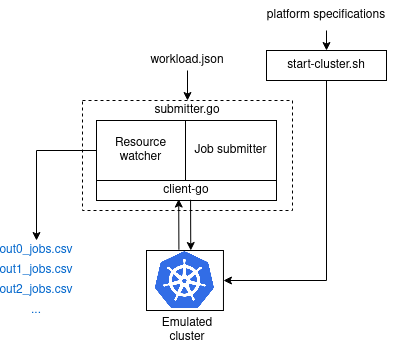
\includegraphics[scale=0.7]{./imgs/prot-k3s.png}
	\caption{An emulated experiment.}
	\label{fig:emulated-expe}
\end{figure}

TODO: scripts to create a cluster with k3s. 

For each workload, run it 10 times for the first two, only a few times for the
last one.

TODO: mention the limit on the amount of cpu and memory as well as the large
experience time. Mention the fact that jobs can't be scheduled across nodes:
if we want to mimic a batch scheduling behavior we need to emulate one big node
containing all the cpu we need (which is not possible), or use adapted workloads.

NOTE: show the graphs? (Gantt charts and aggregated metrics for each wl: makespan, mean waiting time etc. Show the average and standard deviation for these metrics)
\subsection{Simulated testbed}

TODO: Those are the options batkube is run with throughout the experiments.
\begin{itemize}
	\item \texttt{base-simulation-timestep}: 100ms. Starting value for the
		simulation timestep, which then increases with the implemented
		backoff policy. --> Can be the object of an experiment, not
		sure if it impacts the simulation.
	\item \texttt{backoff-multiplier}: 2. Same as last one, not sure if it
		has an impact really.
	\item \texttt{detect-scheduler-deadlock}: true. Obligatory for
		automating experiments
	\item \texttt{scheduler-crash-timeout}: 5s (more than enough)
	\item \texttt{fast-forward-on-no-pending-jobs}: the scheduler is not
		susceptible to reschedule running jobs (there is a de-scheduler
		for that) so we might as well fast forward when there is
		nothing to schedule.
\end{itemize}

The other parameters are precised for each experiment.

\subsection{Studied workloads}

We consider three workloads, representing three different situations. The first
two are simplistic and very controlled, and the last one depicts a more
realistic case. In all cases the required resources are only quantified in cpu
only to simplify the study. Note that Batkube does support memory requets, we
just do not wish to add this other layer of complexity to our experiments.

\begin{itemize}
	\item A \textit{burst} workload, consisting in an important amount of
		jobs submitted at once.  200 delays with duration 170s and
		requesting 1 cpu are submitted at the origin.
	\item A \textit{spaced} workload, where jobs of the same nature are
		submitted at regular intervals.  200 delays with duration 170s,
		and requesting 1 cpu are submitted every 10s.
	\item A \textit{realistic} workload, which is extracted from a larger
		trace of a real system.
\end{itemize}

The first two workloads are straight forward and could be generated with the
use of a plain text editor (understand \texttt{vim} and its macros). The third
workload required more processing to be obtained.  

\subsubsection{Standard Workload Format processing}

First, a trace in standard
workload format (swf) was obtained on a web
archive\footnote{https://www.cs.huji.ac.il/labs/parallel/workload/logs.html}.
The chosen workload was \texttt{KIT-FH2-2016-1.swf} because it is the most
recent and is relatively lightweight. Secondly,
\texttt{evalys}\footnote{https://github.com/oar-team/evalys} allowed us to
extract a subset of this workload lasting for a given period of time and with a
given mean utilization of the resources. We chose a period of 10h with 80\%
utilization of the resources so as to keep reasonable experiment durations --
Later on we experiment with larger workloads to test out Batkube's limits in
terms of scalability.  The third step is translating this extracted workload to
a \texttt{json} file that can be read by Batsim, which is done with a script
written in Go.

After extracting this subset, we are left off with a workload containing jobs
spanning up to 45h and using up to 24048 cpu (or cpu cores), which is undoable
at our scale on our emulated cluster. We need to trim job durations as well as
cpu usage, as we are limited in cpu by the host machine. This is done during
the translation to the \texttt{json} format. The durations are trimmed down to
a maximum of one hour and the cpu usages are normalized so the maximum amount
of cpu requested equals the amount of cpu available per node on the host
machine. Otherwise, the job would be unschedulable which would not present much
interest.

\subsection{Studied platforms and scheduler}

TODO: describe the platform: 16x1cpu for the first two, TBD for the realistic
wl (we run simulations to know what to expect in terms of experiment duration
and adapt the platform so it is not too long).\\


\section{Validation of the simulator outputs}

TODO: With default parameters (timeout TBD with experiments results, max time step same, min delay 0), compare simulated and emulated results. 

Here : the Gantt charts from evalys.

Study on two metrics : makespan and mean\_waiting\_time. Show the box plots for
simulated and emulated metrics.

Discussion:
Container pull and startup time not accounted for in the simulation.

\section{Study of the simulator parameters}

The simulator has a few parameters that impact the simulation speed and
accuracy. The objective is to study the effects of these parameters on the
simulation to better understand the scheduler behavior when running in
coordination with Batkube.\\

The objective here is to fine tune the parameters in order to find a compromise
between accuracy and scalability.

The parameters are:
\begin{itemize}
	\item The \textit{timeout} value when waiting for scheduler decisions.
		Default value: 20ms.
	\item The \textit{minimum delay} we have to spend waiting for the
		scheduler. Default value: 10ms.
	\item The \textit{maximum simulation time step}, which is the maximum
		amount of time Batsim is allowed to jump forward in time.
		Default value: 50s.
\end{itemize}

We first study these parameters one by one by fixing the other parameters to
their default value, then we study what effects these parameters have in
respect to one another, and finally we conduct scalability experiments to test
Batkube's stability and performances on large workloads.

\subsection{Minimum delay}

We observed that not leaving enough time to the scheduler each cycle causes it
to put itself in a deadlock state, or may make batsky-go crash. From there, no
decision is made for the rest of the simulation. 
% The \texttt{detect-scheduler-deadlock} option allows systematically detect such
% crashes based on a timeout value, making Batkube exit the simulation with code
% 1 when it happens.

We expect to see a very high percentage of crashes when this value is low, that
will decrease until there is enough time for the scheduler to make its
computations correctly.\\

For each workload, we compute the crash rate every 5ms, from 0ms to 50ms. Each
point is made by running the simulation 15 times and recording the exit code,
as well as the simulation time. Other parameters: timeout=20ms; max-simulation-timestep=20s.

TODO: 
graph: 

delay vs crash rate

delay vs simulation time in case of success. Two options : mean values with error bars (max \& min values) or overlay the 15 curves.

Note: This issue is resolved with the lastest commits on kubernetes scheduler.
Show the graph for the earlier versions, to warn about this potential issue
with earlier versions of the scheduler\\

For the rest of the experiments, we pick the first minimum delay value that
gets us 100\% success rate (or close to it). So that would be zero, considering
the last note, which is very convenient.

\subsection{Timeout}

Decreasing this value leaves less time for the scheduler to react: for example,
if the scheduler needs 30ms to make a decision upon reception of an update in
the resources state, and the value of the timeout is 20ms, Batkube will receive
the decision on the next cycle which may happen several dozens of seconds later
(depending on the \textit{maximum simulation time step} value). Intuitively,
this will increase the simulation speed while leaving gaps in the decision
process, causing a decrease in accuracy.\\

For each workload we compute the total makespan, the mean waiting time (NOTE:
maybe the stretch but it wouldn't make much sense as delays induced by the
timeout value have nothing to do with the job length) and the simulation
calculation time for a timeout value ranging from 5ms to 50ms, every 1ms. Other
parameters: min-delay=0ms; max-simulation-timestep=20s.

TODO: 
graphs: 

Gantt charts to show the gaps.

timeout vs simulation time

timeout vs makespan: scatter plot, plot a dotted line showing the emulated value. Same for timeout vs mean_waiting_time.


\subsection{Maximum simulation time step}

Having a high maximum time step value will allow Batsim to jump forward further
in time. This may result in skipping scheduler decisions that could have been
made in the mean time, delaying them to when Batsim decides to wake up. We
expect increasing this value to have an analogous effect to the timeout value:
higher simulation speed, but also decreased accuracy due to gaps (delays) in
the decision process.\\

PROTOCOL: same as timeout. max timestep ranges from 1s to 100s with a
logarithmic scale (1s, 2s, \ldots, 9s, 10s, 20s, \ldots, 90s, 100s) Other
parameters: timeout=20ms; min-delay=0ms.

TODO: basically the same graphs as in the timeout

\subsection{Parameters inter dependency}

Studying the parameters independently is not enough, we need to study their
impact relatively to each others.

For instance, the \textit{maximum simulation time step} and the
\textit{timeout} value are tightly linked together regarding their effect on
accuracy. Both decreasing \textit{timeout} and increasing \textit{maximum
simulation time step} will increase the amount of delays in the decision making
of the scheduler, but also their length, multiplying the impact on accuracy.

On the other hand, we do not except the \textit{minimum wait delay} to have any
impact other than increasing the simulation stability.

PROTOCOL: We know the simulations are statistically the same by now, and we're
confident enough to run only one simulation per point. Timeout value ranges
from 5ms to 50ms, max timestep ranges from 1s to 100s (logarithmic again).

TODO: Facet graphs: timestep vs timeout vs accuracy vs simulation time. We can
define accuracy as one on the euclidean distance between emulated and simulated
makespan and mean waiting time: \[\frac{1}{\sqrt{(makespan_{sim} -
	makespan_{emu})^2 + (waitingtime_{sim} - waitingtime_{emu})^2}}\]

\section{Scalability experiments and scheduler limits}

We have extracted a few workloads recorded on real systems to test out the
scheduler performances in regard to scalability, that is to say the ability to
run large workloads in a minimal amount of time.

PROTOCOL: go all out on large workloads and platform

TODO: on small workloads the scheduler tends to over allocate when it is not supposed
to: same behavior in emulation and simulation

\backmatter
\printbibliography
\end{document}
